%!TEX root = ../doc.tex
\chapter{Fundamentals}
\label{sec:Fundamentals}
The following chapter describes methods and technologies that are used within this thesis.
\section{Mathematics for Rotation and Translation}
\label{sec:LinAlgRotation}
Augmented reality relies on having accurate positional and angular information to estimate the required size and warp of a virtual object projected into the real world. A MEMS module containing a gyroscope and an accelerometer provides rotation and acceleration information to the system to assist the positional tracking. 
\subsection{Euler Rotations and Linear Algebra}
A common way to calculate rotations and translations are matrix-vector multiplications. The standard matrices for rotating with the angle $\phi$ around $X$, $Y$ and $Z$ are shown in the following:
\begin{equation*}
    A_{rot,X} = 
    \begin{bmatrix}
    1 & 0 & 0 \\
    0 & cos \phi & -sin \phi \\
    0 & sin \phi & cos \phi
    \end{bmatrix}
    \quad
    A_{rot,Y} = 
    \begin{bmatrix}
    cos \phi & 0 & sin \phi \\
    0 & 1 & 0 \\
    -sin \phi & 0 & cos \phi
    \end{bmatrix}    
    \quad
    A_{rot,Z} = 
    \begin{bmatrix}
    cos \phi & sin \phi & 0 \\
    -sin \phi & cos \phi & 0 \\
    0 & 0 & 1
    \end{bmatrix} 
\end{equation*}
A combination of the three matrices leads to a rotation matrix with a rotation axis that is not strictly bound to $X$, $Y$, or $Z$. Matrix multiplication is not commutative, so the order of the multiplications matters. In the following example, the vector gets rotated first around $X$, then $Y$, and around $Z$ in the end. This chain of matrix operations is read from right to left in the equation.
\begin{equation*}
    A_{rot} = 
    \begin{bmatrix}
    a_{0,0} & a_{0,1} & a_{0,2}  \\
    a_{1,0} & a_{1,1} & a_{1,2}  \\
    a_{2,0} & a_{2,1} & a_{2,2} 
    \end{bmatrix}
    =A_{rot,Z} \cdot A_{rot,Y} \cdot A_{rot,X}
\end{equation*}
With this matrix, a three dimensional vector can be rotated at once around an arbitrary axis for the desired angle. Applying this transformation to each vertex of a virtual 3D object results in a rotation of the whole object around the origin $(0,0,0)$.\\
\begin{equation*}
    \begin{pmatrix}
    x'  \\
    y'  \\
    z' 
    \end{pmatrix} 
    = 
    \begin{bmatrix}
a_{0,0} & a_{0,1} & a_{0,2}  \\
a_{1,0} & a_{1,1} & a_{1,2}  \\
a_{2,0} & a_{2,1} & a_{2,2} 
\end{bmatrix}
\cdot 
\begin{pmatrix}
    x  \\
    y  \\
    z 
    \end{pmatrix}
\end{equation*}
To avoid using an inhomogenous linear system for moving an object, a fourth dimension is needed. By extending the vectors with a $1$ and using the fourth column in the matrix to alter $X$, $Y$ and $Z$, these vector entries can be moved without applying any rotation. 
\begin{equation*}
    \begin{pmatrix}
        x+\Delta X  \\
        y+\Delta Y  \\
        z+\Delta Z  \\
        1
        \end{pmatrix} 
        = 
    \begin{pmatrix}
    x'  \\
    y'  \\
    z'  \\
    1
    \end{pmatrix} 
    = 
    \begin{bmatrix}
1 & 0 & 0 & \Delta X \\
0 & 1 & 0 & \Delta Y  \\
0 & 0 & 1 & \Delta Z  \\
0 & 0 & 0 & 1
\end{bmatrix}
\cdot 
\begin{pmatrix}
    x  \\
    y  \\
    z  \\
    1
    \end{pmatrix}
\end{equation*}
To combine the rotation matrix with the translation matrix, the 3x3 rotation matrix gets placed top-left into the 4x4 unit matrix. Now, the rotation matrix also being a 4x4 matrix, rotations and translations can be chained up following the common laws of linear algebra. Chaining up translations and rotations allows moving the rotation axis for an object.
\begin{equation*}
    \begin{pmatrix}
    x'  \\
    y'  \\
    z'  \\
    1
    \end{pmatrix} 
    = 
    \begin{bmatrix}
a_{0,0} & a_{0,1} & a_{0,2} & 0 \\
a_{1,0} & a_{1,1} & a_{1,2} & 0 \\
a_{2,0} & a_{2,1} & a_{2,2} & 0 \\
0 & 0 & 0 & 1
\end{bmatrix}
\cdot 
\begin{pmatrix}
    x  \\
    y  \\
    z  \\
    1
    \end{pmatrix}
\end{equation*}
The dependency on the order of the rotations poses a problem visualized in image \ref{im:EulerRotation}: The values returned by a gyroscope would need to be applied all at once and not one after another. 
\begin{figure}[H]
	\centering
		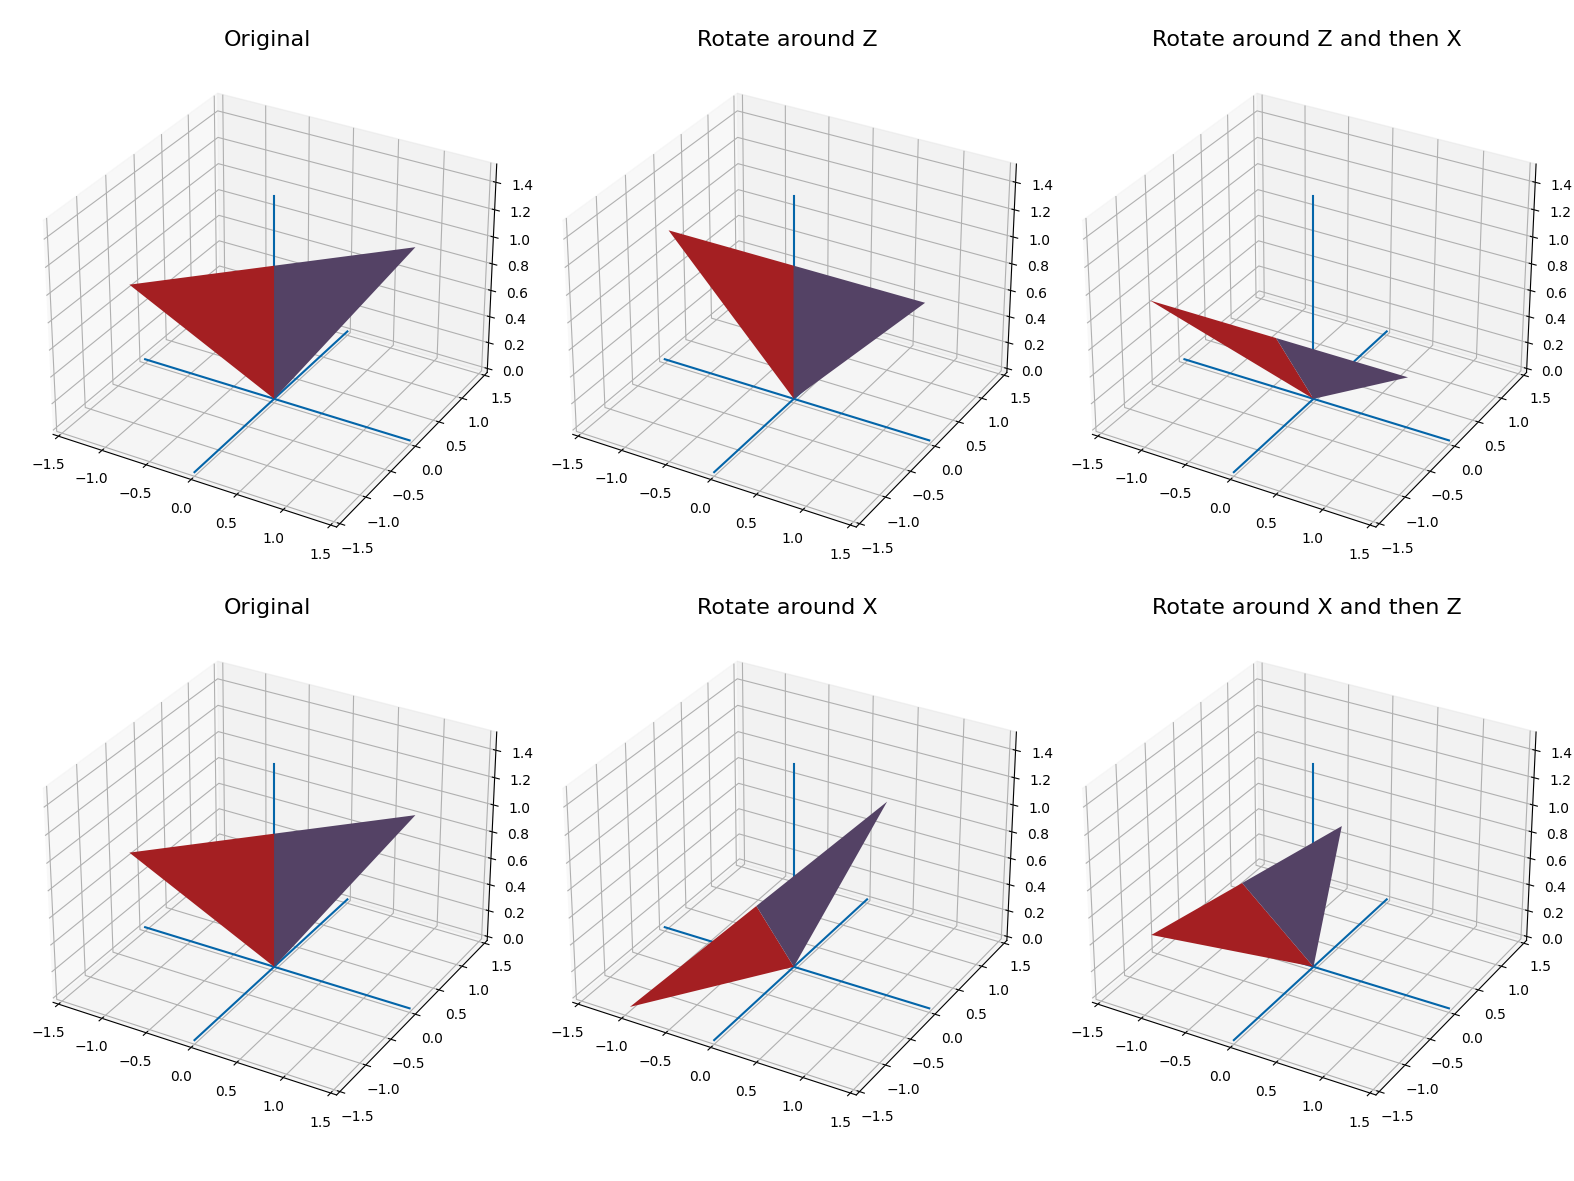
\includegraphics[width=1.0\textwidth]{images/euler_rotation.png}
	\caption{Euler rotations are dependent on the order of the individual rotations. Rotating around X and then Z results in a different outcome, than first rotating around Z and then X.}
	\label{im:EulerRotation}
\end{figure}
\subsection{Standard Vulkan Coordinate System}
In Vulkan, every vertex coordinate of a 3D rendered object gets mapped to the nearest pixel in the viewport window. This vertex mapping is done in multiple steps from "view coordinates" via "clip coordinates" towards "normalized device coordinates" to the "pixel coordinates".\\
A 3D object is a cloud of vertex coordinates described by a list three-dimensional vectors $\overrightarrow{v_{v}} = (x_{v},y_{v},z_{v})$ (the subscript $v$ denotes the "view coordinates"). These coordinates usually do not contain data regarding the whole object's scale, position, and rotation in 3D space - this information is added with matrices in the shader step.\\
Vulkan expects the output of the shader step to be in clip coordinates. Clip coordinates are four-dimensional vectors $\overrightarrow{v_{c}} = (x_{c},y_{c},z_{c},w_{c})$ (the subscript $c$ denotes the "clip coordinates") and the result of a matrix multiplication operation.\\
\begin{equation*}  
    \overrightarrow{v_{c}} = A \cdot  \overrightarrow{v_{v}}
\end{equation*}
\begin{equation*}
    \begin{pmatrix}
    x_{c}  \\
    y_{c}  \\
    z_{c}  \\
    w_{c}
    \end{pmatrix} 
    = 
    \begin{bmatrix}
a_{0,0} & a_{0,1} & a_{M 0,2} &  a_{0,3} \\
a_{1,0} & a_{1,1} & a_{M 1,2} &  a_{1,3} \\
a_{2,0} & a_{2,1} & a_{M 2,2} &  a_{2,3} \\
a_{3,0} & a_{3,1} & a_{M 3,2} & a_{3,3}
\end{bmatrix}
\cdot 
\begin{pmatrix}
    x_{v}  \\
    y_{v}  \\
    z_{v}  \\
    1
    \end{pmatrix}
\end{equation*}
Generally, three combined matrix multiplications describe how a 3D object is rendered – the model matrix, the view matrix, and an added projection matrix. The model matrix ($A_{Model}$) defines the scale, rotation and position of the 3D object and is a standard 4x4 matrix as explained in section \ref{sec:LinAlgRotation}.\\ 

The view matrix ($A_{View}$) is also is a rotation and translation matrix, but describes the position and direction of the viewport camera (or eye). Rotating the camera rotates the rendered virtual space, which indirectly moves and turns the models in the viewport. The linmath-library offers the "4x4\_look\_at" function that calculates the view matrix based on camera position, a viewing angle, and the information regarding the "upwards" direction.\\
The projection matrix ($A_{Projection}$)  is not a rotation and translation matrix besides the model and the view matrix. As its name suggests, the projection matrix reduces the vertex' 3d coordinates to the viewport plane by projecting them onto a virtual screen. By taking a field of view angle, the projection matrix allows camera distortion. The linmath-library offers the "4x4\_perspective" function that calculates the projection matrix based on a given field of view angle 
Within the vertex shader, these three matrices are chained to perform the desired transformation.
\begin{equation*}  
    A = A_{Projection} \cdot A_{View} \cdot A_{Model}
\end{equation*}
By division of the clip coordinate components $x_{c}$, $y_{c}$ and $z_{c}$ with $w_{c}$, Vulkan itself calculates the normalized device coordinates $\overrightarrow{v_{NDC}} = (x_{NDC}, y_{NDC}, z_{NDC})$.
\begin{equation*}
    \begin{pmatrix}
    x_{NDC}  \\
    y_{NDC}  \\
    z_{NDC}  \\
    \end{pmatrix} 
    =
    \begin{pmatrix}
        \frac{x_{c}}{w_{c}}  \\
        \frac{y_{c}}{w_{c}}  \\
        \frac{z_{c}}{w_{c}}  \\        
        \end{pmatrix}     
\end{equation*}
The transformation to the pixel coordinates are also done by Vulkan without requiring any action by the developer. The only noticable detail is the alignment of the normalized device coordinates. On the viewport surface, the point $(0 / 0)$ is located in the center. Top left is $(-1 / -1)$, top right is $(1 / -1)$, bottom left is $(-1 / 1)$ and bottom right is $(1 / 1)$.

\subsection{Rotation with Quaternions}
Quaternions - also known as "Hamilton Numbers" - are the three dimensional equivalent to complex numbers. Analogue to complex numbers, quaternions also consist of a real part, but add three imaginary parts $\textbf{i}$, $\textbf{j}$ and $\textbf{k}$. Most often, quaternions get represented in the form $a+b\textbf{i}+c\textbf{j}+d\textbf{k}$ or a four dimensional vector $(a, b, c, d)$